O objetivo deste capítulo é mostrar os conceitos envolvidos no paradigma de computação distribuída, mais especificamente os de Computação em Nuvem, abordando suas características e suas particularidades. Também descreve as chamadas Federações de Nuvens Computacionais e como este trabalho pretende utilizá-las para integrar um Sistema Gerenciador de \textit{Workflows} Científicos à atual plataforma do BioNimbuZ. Para isso, a Seção \ref{cap2sec1} mostra o histórico da computação distribuída e seus principais elementos (como \textit{Grids} e \textit{Clusters}), a Seção \ref{cap2sec2} apresenta os conceitos básicos que norteiam o entendimento sobre nuvens computacionais, mostrando como diversas pesquisas contribuíram para o conceito atual desta tecnologia. Por fim, a Seção \ref{cap2sec3} mostra os detalhes da chamada Federação de Nuvens Computacionais, quais seus objetivos, suas características e o que a distingue dos outros modelos de computação distribuídas. 

\section{Sistemas Distribuídos} \label{cap2sec1}

A Internet é utilizada por bilhões de pessoas com vários propósitos diferentes, como ler e-mails, visualizar conteúdo multimídia, fazer compras ou apenas realizar uma busca por um assunto de interesse. Isso passa ao usuário a ilusão de que a informação e o sistema que a provê se encontram localmente em sua máquina. Mas, a Internet representa um enorme sistema distribuído que se parece como um recurso único disponível em um conjunto mínimo de configuração de conexão e em apenas poucos cliques \cite{cloud_360}.

O conceito de sistema distribuído possui diversas definições e pontos de vista. Colouris [7] define um sistema distribuído como ``um sistema em que componentes de hardware e software comunicam e coordenam suas ações apenas trocando mensagens''; Por outro lado, Tanenbaum [8] o define como ``uma coleção de computadores independentes que aparecem ao usuário do sistema como um único computador''. E Keith Marzullo [9], define um sistema distribuído como ``Uma coleção de processos sequenciais $P_1, P_2, ..., P_n$ e uma rede capaz de implementar canais de comunicação unidirecionais entre pares de processos para troca de mensagem''. 

Dessa forma, as definições convergem para um conjunto de aspectos comuns e essencias que nos ajuda a distinguir sistemas distribuídos: 

\begin{itemize}
    \item São formados por um conjunto de computadores (ou unidades de processamento);
    \item São conectados por uma rede, sua comunicação é feita através de troca de mensagens e, portanto, não compartilham memória;
    \item São vistos pelos usuários como um recurso único (transparência [8]);
    \item Facilitam a utilização de recursos por usuários (ou aplicações);
    \item São escaláveis, isto é, possibilitam o aumento ou a diminuição de usuários ou recursos de maneira facilitada;
    \item Possuem desafios de temporização e sincronização.
    
    Assim, embora seja possível perceber os desafios inerentes à implementação deste tipo de sistema, o ganho de poder computacional vale à pena esse esforço.
\end{itemize}

Nas próximas Seções serão apresentados os conceitos e principais aspectos de um \textit{Cluster} computacional e Computação em \textit{Grid}, os quais são tidos como base para o conceito de Nuvem Computacional.

\subsection{\textit{Cluster} Computacional} \label{cap2sec1subsec1}

A primeira iniciativa na construção do conceito e implementação de \textit{Clusters} Computacionais foi realizada pela IBM em meados dos anos 60 como alternativa de interligar grandes \textit{Mainframes} para prover aos seus usuários uma forma comercial mais eficiente de paralelismo. Contudo, o conceito de clusterização não ascendeu como previsto até o surgimento de outras três tecnologias: microprocessadores de alta-performance, redes de alta velocidade e protocolos para computação distribuída de alta-performance [13]. 

Os recentes avanços dessas três tecnologias, somadas à sua acessibilidade (baixo preço decorrente da alta demanda) facilitaram a implementação de \textit{clusters} computacionais como solução do antigo problema da eficiência de custos na busca de sistemas paralelos de alta performance. Para se construir um \textit{cluster}, os computadores componentes devem ter alguns elementos essenciais [14]:

\begin{itemize}
    \item Vários computadores de alta performance (PCs, \textit{Workstations}, \textit{Mainframes});
    \item Sistemas Operacionais;
    \item Conectados por uma rede de alta performance (como \textit{Gigabit Ethernet});
    \item \textit{Middleware} de gerenciamento de \textit{Clusters} (serviços e abstrações que facilitam o desenvolvimento de aplicações distribuídas. O \textit{middleware} permite ao \textit{cluster} manter a uniformidade na presença de diferentes hardwares e SOs);
    \item Ambiente de computação paralela;
    \item Aplicações.
\end{itemize}

A Figura \ref{fig:cluster_architecture} apresenta a arquitetura conceitual de um \textit{cluster}, mostrando suas camadas e alguns dos elementos descritos acima:

\begin{figure}[H]
	\centering
	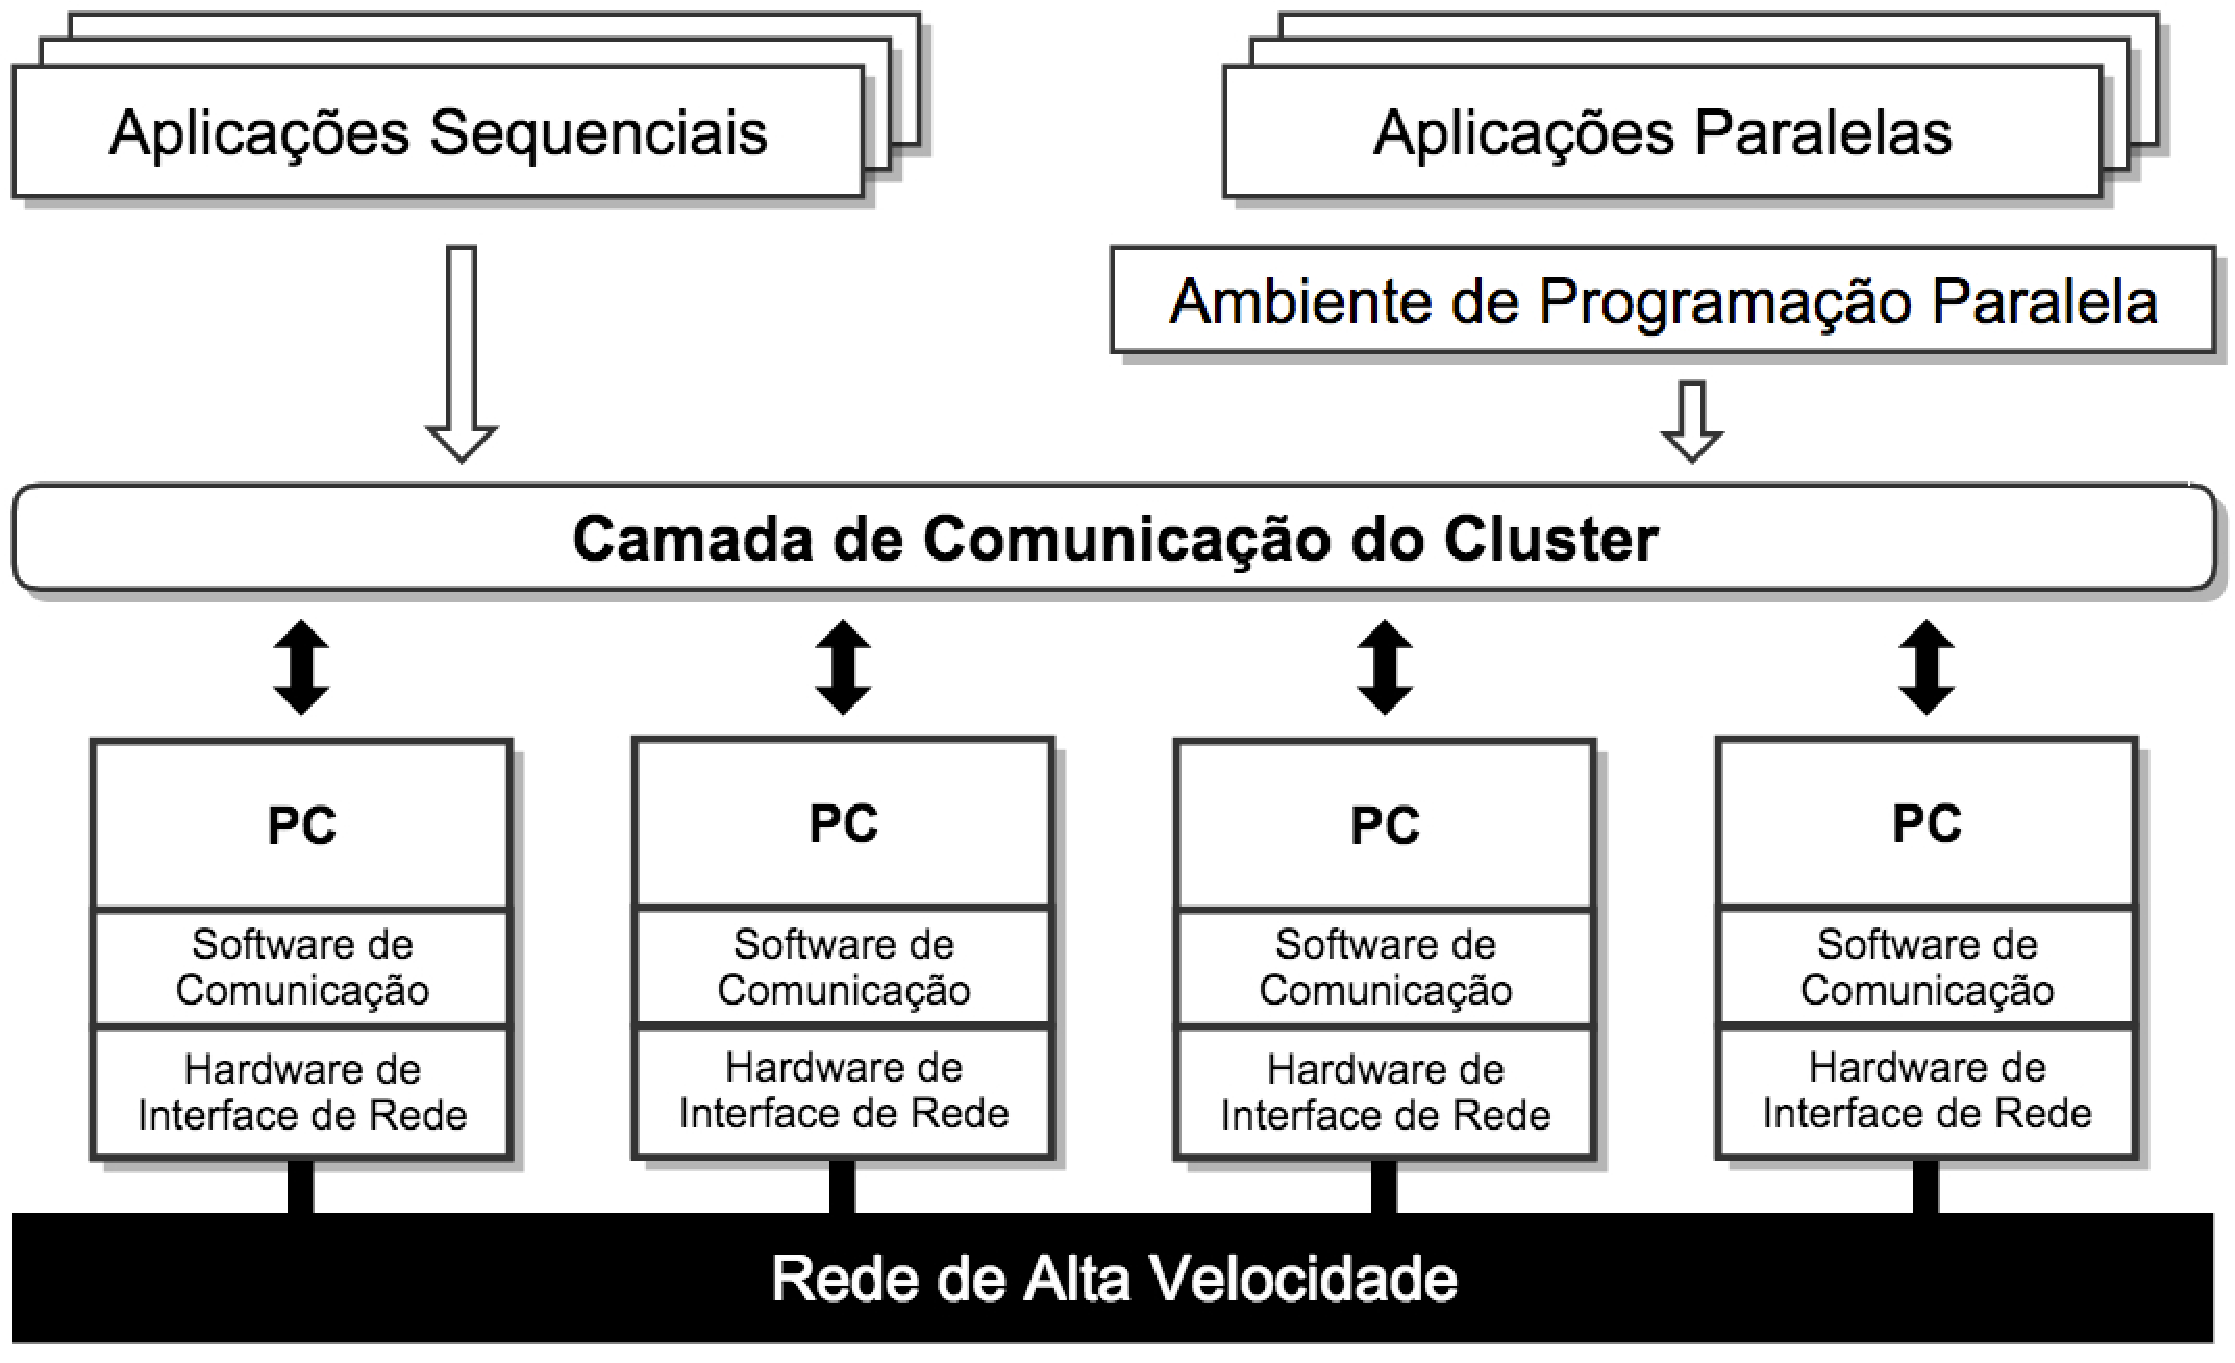
\includegraphics[scale=0.4]{arquitetura_cluster.pdf}
	\caption{Arquitetura de um \textit{Cluster}.}
	\label{fig:cluster_architecture}
\end{figure}

Na busca para provar o ganho de performance de \textit{clusters} sobre as plataformas tradicionais de sistemas distribuídos, diversos projetos acadêmicos surgiram, como o Beowulf [14], Berkeley NOW [15] e HPVM [16].

Beowulf foi um \textit{cluster} construído em 1994 por Thomas Sterling e Don Becker e consistia de 16 processadores DX4 conectados por um canal Ethernet, dedicados à programação paralela [14]. O \textit{cluster} criado foi muito bem visto pela área acadêmica e comercial, tanto que a NASA se interessou por este novo modelo. Em pouco tempo, o \textit{cluster} Beowulf foi bastante difundido, tornando-se “Projeto Bewoulf” e passou a ser visto como gênero dentro da comunidade de Computação de Alta Performance (\textit{High Performance Computing}).

Berkeley NOW (\textit{Network of Workstations}) difere do \textit{cluster} Beowulf pois seus nós computacionais são computadores completos - computadores pessoais com teclado, mouse e som - conectados pela Internet (os nós de um \textit{cluster} Beowulf são nós especializados, \textit{workstations} que ficam dia e noite apenas processando informações relacionadas ao \textit{cluster}, não servindo, portanto, como um computador pessoal). Na maioria dos casos, nós NOW são utilizados para processamento a noite ou nos fins de semana, quando não estão sendo acessados pelos usuários, ou durante o dia, quando o \textit{cluster} utiliza parte do poder de processamento do computador pessoal do usuário, utilizando ciclos ociosos de CPU e agregando-os pela Internet. 

Esse modelo de computação distribuída tinha diversas limitações quanto ao tipo de aplicação que poderia ser executado no cluster NOW. Nesse contexto, o \textit{cluster} Bewoulf tinha um melhor desempenho pois possuía as seguintes características:

\begin{itemize}
    \item Utilizava processadores dedicados;
    \item Utilizava redes privadas de alta performance;
    \item Seu software era customizável;
    \item Softwares podiam ser clonados e enviados pela internet.
\end{itemize}

\subsection{\textit{Grid} Computacional} \label{cap2sec1subsec2}

Em meados dos anos 90 o termo \textit{Grid} Computacional foi criado para descrever tecnologias que possibilitariam usuários obterem poder computacional sobre demanda, assim como a energia é disponibilizada pela rede elétrica. Distingue do modelo tradicional de computação distribuída pelo foco em compartilhamento de grandes quantidades de recursos e, geralmente, por ser orientado à computação de alta performance. É uma forma de computação que envolve coordenar e compartilhar recursos computacionais, aplicações, dados, armazenamento e/ou recursos de rede através de sistemas dinâmicos e geograficamente dispersos [11], de maneira flexível, segura e coordenada servindo às chamadas Organizações Virtuais [12]. Uma Organização Virtual é um conjunto de indivíduos e/ou instituições interessados em acessar diretamente máquinas, software, dados e outros recursos. Esse compartilhamento é extremamente controlado, com regras definindo o que está, com quem e as condições daquilo que está sendo compartilhado.

Um sistema gerenciador de um \textit{Grid} Computacional não está somente voltado ao processamento de dados, mas também ao gerenciamento de recursos de todo o sistema, seja ele software (aplicações, protocolos, sistemas operacionais) ou hardware (armazenamento, consumo de CPU, utilização de memória). Foster \textit{et al.} \cite{cloud_360} dividem sua arquitetura em 5 camadas, tomando como base a arquitetura do Protocolo de Internet (\textit{Internet Protocol}). Essa arquitetura é apresentada na Figura \ref{fig:grid_architecture}, na qual estão presentes as seguintes camadas: 

\begin{figure}[h!]
	\centering
	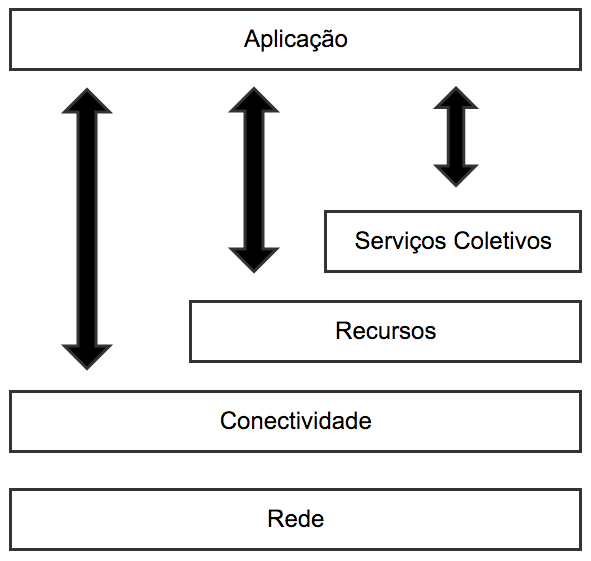
\includegraphics[scale=0.45]{arquitetura_grid.png}
	\caption{Arquitetura de um \textit{Grid}, adaptado de \cite{cloud_360}.}
	\label{fig:grid_architecture}
\end{figure}

\begin{itemize}
	\item \textbf{Camada de Rede:} Fornece acesso compartilhado aos recursos computacionais a partir dos protocolos de \textit{Grid}. Um recurso pode ser uma entidade lógica, como um sistema de arquivos distribuídos, por exemplo um \textit{cluster}.
	\item \textbf{Camada de Conectividade:} Define o método de comunicação e protocolos de autenticação para transações especifícas da rede interna do \textit{Grid}. Além disso, provê mecanismos de segurança criptográfica para verificar a identidade de usuários e recursos.
	\item \textbf{Camada de Recursos:} Define protocolos para transações, inicialização, monitoração, controle e custos de operações que utilizam recursos individuais. Esta camada se preocupa apenas com o seu conjunto de recursos, não se importando com o estado global dos recursos compartilhados.
	\item \textbf{Camada de Serviços Coletivos:} Enquanto a Camada de Recursos está ligada à interações com recursos únicos, a Camada de Serviços Coletivos tem o objetivo de capturar e gerenciar transações entre conjuntos de recursos.
	\item \textbf{Camada de Aplicação:} A última camada na arquitetura de Grids abrange as aplicações que operam dentro do ambiente de uma Organização Virtual, ou seja, esta camada está preocupada nas aplicações clientes que são executadas dentro de um grupo que compartilha o mesmo recurso.
\end{itemize}

Na próxima Seção serão apresentados os principais conceitos sobre Nuvens Computacionais, além das definições presentes na bibliografia, suas vantagens e desvantagens sobre os modelos de computação distribuída mostrados nessa Seção.

\section{Nuvem Computacional} \label{cap2sec2} 

Com o rápido desenvolvimento de tecnologias de processamento e de armazenamento de dados e o crescimento da Internet, recursos de computação tornaram-se mais acessíveis, mais poderosos e mais disponíveis do que nunca. Essa tendência tecnológica permitiu a realização de um novo modelo de computação chamada computação em nuvem, em que os recursos computacionais (CPU, rede, memória, armazenamento) são fornecidos como serviços que podem ser alugados e liberado pelos usuários através da Internet em um modelo sob-demanda. Esse conjunto de tecnologias provê aos usuários uma gama enorme de opções de usos dessa nova plataforma. Com ela, os serviços são disponibilizados de forma transparente, representando uma nova maneira de se utilizar recursos computacionais. 

A ideia principal por trás da computação em nuvem não é exatamente nova. Em meados dos anos 60, John McCarthy já havia previsto que o modelo de computação seria provido ao público de uma maneira similar ao que acontece nas redes elétricas, por exemplo. Isso aconteceu quando grandes empresas capazes de implantar enormes \textit{datacenters} a custos competitivos resolveram adotar esse novo paradigma da computação. Em 2006, o termo ``nuvem'' ganhou popularidade quando o CEO (\textit{Chief Executive Officer}) da Google, Eric Schmidt, o utilizou para descrever o modelo de negócios para prestação de serviços pela internet. Desse momento em diante, o termo ``nuvem'' realmente começou a ficar popular com ações de \textit{marketing} e com o nascimento de diversas empresas especializadas. 

A partir deste ponto, diversas definições surgiram em busca de um padrão para o conceito de computação em nuvem. Foster \textit{et al.} \cite{cloud_360} a definem como um paradigma de computação distribuída em larga escala movida pela economia da indústria, na qual um grande conjunto de recursos computacionais são providos sob-demanda a usuários externos pela Internet. Isso reforça a ideia de McCarthy de computação provida como serviços. Armburst \textit{et al.} [17] trazem a definição de computação em nuvem como a união das aplicações disponibilizadas como serviços pela Internet e o hardware nos \textit{datacenters} que as provém. 

NIST (\textit{National Institute of Standards and Technology}) a define como ``um modelo que possibilita o acesso ubíquo, conveniente, sob-demanda a um conjunto configurável de recursos computacionais (redes, servidores, armazenamento, aplicações, seviços) que podem ser rapidamente provisionados e liberados com um esforço mínimo de gerenciamento ou interação do provedor de serviço'' [16]. 

Na indústria de Tecnologia da Informação (TI), o surgimento do modelo de Computação em Nuvem tem causado um enorme impacto nos últimos anos, onde grandes empresas como Google [45], Amazon [46] e Microsoft [47] se esforçam para fornecer plataformas de nuvem cada vez mais poderosas, disponíveis, de confiança e com melhor custo-benefício. Ao mesmo tempo, empresas procuram reformular seus modelos de negócios para se utilizarem dos benefício deste novo paradigma. Dessa forma, a computação em nuvem fornece vários recursos interessantes que a torna atraente para empresas, tais como [5]:

\begin{itemize}
	\item \textbf{Não necessita de investimento inicial}: A computação em nuvem usa um modelo de precificação em que o usuário paga apenas pelo recurso computacional utilizado. Um prestador de serviço não precisa investir na infraestrutura para começar a se utilizar dos ganhos tecnológicos de uma nuvem computacional. Ele simplesmente aluga os recursos de acordo com suas próprias necessidades e paga por aquilo que utilizar.
	\item \textbf{Reduz o custo operacional:} Recursos em um ambiente de nuvem podem ser rapidamente alocados e desalocados sob-demanda. Assim, um prestador de serviços não precisa  mensurar sua capacidade de acordo com a carga de pico (carga máxima). Isso proporciona uma enorme economia uma vez que os recursos podem ser liberados para economizar custos de serviço quando a demanda for baixa.	
	\item \textbf{Altamente escalável:} Provedores de infraestrutura possuem grandes quantidades de recursos a partir de \textit{datacenters} e os tornam facilmente acessíveis. Um provedor pode facilmente expandir sua capacidade, a fim de lidar com um rápido aumento na carga de serviço.	
	\item \textbf{Acessibilidade:} Serviços hospedados na nuvem são geralmente baseado na \textit{web}. Assim, são facilmente acessíveis através de uma grande variedade de dispositivos com conexões de Internet. Estes dispositivos não só incluem computadores \textit{desktop} e \textit{notebooks}, mas também celulares e \textit{tablets}.
	\item \textbf{Reduz os riscos de negócios e despesas de manutenção}: Por terceirizarem os serviços de infraestrutura para as nuvens, prestadores de serviços transferem os riscos empresariais (tais como falhas de hardware) para os provedores de infraestrutura, que muitas vezes tem um maior conhecimento e estão melhor equipados para o gerenciamento desses riscos.
\end{itemize}

No entanto, embora a computação em nuvem tenha mostrado consideráveis oportunidades para a indústria de TI, também traz muitos desafios únicos que precisam ser cuidadosamente abordados, tais como confidencialidade das informações, integridade de dados, disponibilidade dos serviços, tolerância a falhas e um dos pontos mais discutidos que é a segurança. 

\subsection{Tipos de Nuvens} \label{cap2sec2subsec2}

As nuvens computacionais podem ser divididas em quatro tipos diferentes de implantação [16]: nuvens públicas, privadas, comunitárias ou híbridas, as quais são descritas a seguir: 

\begin{itemize}
	\item \textbf{Nuvens Públicas: } Sua infraestrutura é disponibilizada para o público em geral, mantida e gerenciada por uma instituição acadêmica, comercial ou governamental e não impõe condições para sua utilização. Seus recursos computacionais são provisionados dinamicamente e são acessíveis através da Internet (geralmente, com a utilização de \textit{webservices}).
	\item \textbf{Nuvens Privadas: } A utilzação da infraestrutura desse tipo de nuvem é exclusivo de uma única companhia ou grupo de empresas, compreendendo múltiplos usuários. Seu gerenciamento pode ser feito pela própria instituição, por outra empresa ou pela junção de ambas as partes.
	\item \textbf{Nuvens Comunitárias: } Esse tipo de nuvem é provisionado para a utilização exclusiva de uma comunidade específica de consumidores de uma organização com interesses em comum (por exemplo, organizações com o mesmo requisito em segurança, mesmos requisitos em performance). Sua implantação pode ocorrer dentro ou fora da organização.
	\item \textbf{Nuvens Híbridas: } Esse tipo de infraestrutura é uma composição de dois ou mais tipos de nuvens (públicas, privadas ou comunitárias) em que o provedor de serviços disponibiliza tecnologias proprietárias que permitem portabilidade de dados e aplicações entre as nuvens que a compõe. Essa infraestrura é muito útil quando, por exemplo, se quer trafegar dados sensíveis e sigilosos em um ambiente controlado e gerenciado internamente (utilização de uma nuvem privada), enquanto outros dados e aplicações podem trafegar em nuvens públicas ou comunitárias.
\end{itemize}

\subsection{Arquitetura} \label{cap2sec2subsec3}

A arquitetura de uma nuvem computacional pode ser dividida em quatro camadas distintas \cite{cloud_360}[15]: camada de hardware (também chamada de camada de \textit{datacenter}), camada de infraestrutura, camada de plataforma e a camada de aplicação. Elas podem ser descritas da seguinte maneira:

\begin{itemize}
	\item \textbf{Camada de Hardware:} Esta camada é responsável pela gestão dos recursos físicos da nuvem, incluindo servidores, roteadores, \textit{switches}, sistemas de energia e refrigeração. Na prática, a camada de hardware é implementada em enormes centros de dados (\textit{datacenters}), os quais geralmente contém milhares de servidores organizados em \textit{racks} e interconectado através de \textit{switches}, roteadores ou outros dispositivos de rede. Problemas típicos na camada de hardware incluem configuração de hardware, tolerância a falhas, gestão, monitoração e refrigeração.
    \item \textbf{Camada de Infraestrutura:} Também conhecida como a camada de virtualização (\textit{virtualization layer}). A camada de infraestrutura cria um \textit{pool} de armazenamento e recursos de computação por meio do compartilhamento dos recursos físicos que utilizam tecnologias de virtualização como o Xen [17], o KVM [18] e o VMware [19]. A infraestrutura é uma camada essencial da computação em nuvem, uma vez que muitas características chaves, tais como a atribuição dinâmica de recursos, são apenas disponibilizados através de tecnologias de virtualização.
    \item \textbf{Camada de Plataforma:} Construída no topo da camada de infraestrutura, a camada de plataforma consiste de sistemas operacionais e \textit{frameworks} de aplicação. A finalidade da camada de plataforma é minimizar o ônus da implantação de aplicativos diretamente em \textit{containers} VM (método em que a camada de virtualização é executada dentro do sistema operacional em que reside).
    \item \textbf{Camada de Aplicação:} Reside no nível mais alto da hierarquia, a camada de aplicação consiste nas aplicações reais sendo executadas em nuvem. Diferentes de aplicações tradicionais, aplicações em nuvem podem aproveitar o recurso de escalonamento automático para alcançar melhor desempenho, disponibilidade e custo operacional mais baixo.
\end{itemize}

\subsection{Modelos de Serviço} \label{cap2sec2subsec4}

A computação em nuvem emprega um modelo de negócios orientado a serviços, ou seja, recursos de hardware e software são disponibilizados sob-demanda. Conceitualmente, cada camada da arquitetura descrita na Seção \ref{cap2sec2subsec3} pode ser implementada como um serviço à camada acima. Em outras palavras, a camada acima será a consumidora dos serviços providos pela camada imediatamente abaixo. Esse modelo em camadas está descrito na Figura \ref{fig:cloud_architecture}.

\begin{figure}[H]
	\centering
	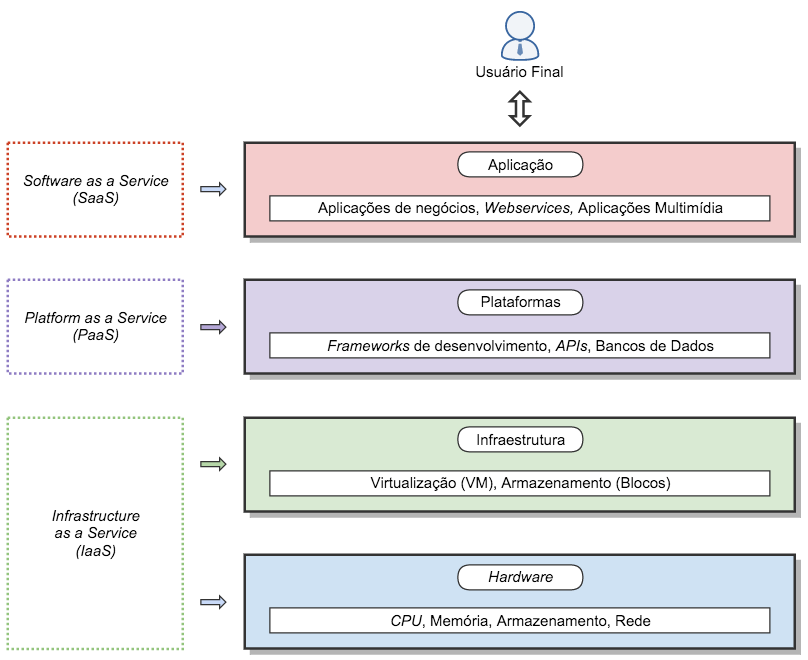
\includegraphics[scale=0.54]{arquitetura_nuvem.png}
	\caption{Arquitetura de uma Nuvem Computacional [15].}
	\label{fig:cloud_architecture}
\end{figure}

Esses serviços são categorizados no seguintes três modelos \cite{cloud_360}[5][15]: 

\begin{itemize}
	\item \textbf{\textit{Infrastructure-as-a-Service}} (IaaS): provê recursos computacionais ao usuários, tais como poder computacional, armazenamento de dados e redes virtuais para que possam implantar e executar qualquer tipo de software. A tecnologia de virtualização é essencial para este modelo, pois dá ao provedor deste serviço a habilidade de que vários usuários possam compartilhar recursos de uma mesma máquina física. Exemplos de provedores deste modelo são: Amazon EC2 [28], Google Compute Engine [48] e GoGrid [49].
	\item \textit{\textbf{Platform-as-a-Service}} (PaaS): Dá ao consumidor deste serviço a capacidade de implantar aplicações criadas pelo usuário ou adquiridas de terceiros, criadas a partir de linguagens de programação, bibliotecas de software, \textit{APIs} (\textit{Application Programming Interface}) e ferramentas suportadas pelo provedor. Nesse modelo, o usuário não gerencia aspectos do hardware e do software necessários para execução da infraestrutura da nuvem. Alguns exemplos são: Heroku [29], CloudForge [50] e AppScale [51].
	\item \textit{\textbf{Software-as-a-Service}} (SaaS): Provê aplicações que estão sendo executadas em algum ponto da Internet por um provedor IaaS, eliminando a necessidade de instalar e executar a aplicação no computador do usuário. São independentes de plataforma e geralmente provêem uma interface para que o usuário possa acessar e utilizar esse serviço. Algumas empresas que implementam esse modelo de serviço são: Abiquo [52], SalesForce [53] e Zendesk [54]. 
\end{itemize}

A próxima Seção traz os conceitos de um novo modelo de estrutura de nuvens computacionais, a federação de nuvens, a qual traz inovações e satisfaz necessidades trazidas pelos modelos de nuvem descrito nesta Seção. 

\section{Federação de Nuvens} \label{cap2sec3}

Com o passar dos anos, diversas necessidades surgiram no contexto da computação em nuvem e a sua utilização de forma isolada passou a não ser mais suficiente para algumas aplicações. Assim, medidas foram tomadas como forma de suprí-las, tais como a criação de \textit{datacenters} espalhados ao redor do mundo para a aumentar a tolerância a falha de suas aplicações, prevendo possíveis quedas de seus servidores e a redundância de dados, visando manter a taxa de disponibilidade dos serviços providos. Dessa forma, integrar diferentes serviços de nuvens para continuar atendendo às expectativas de qualidade de serviço (\textit{QoS - Quality of Service}) passou a ser um requisito necessário para continuar fornecendo serviços de forma rápida, eficiente e escalável. 

Assim, a federação de nuvens é uma área de pesquisa interessante na computação em nuvem e está muito focada na continuidade do \textit{QoS}, empenhando-se no desenvolvimento de mecanismos para manter o serviço disponibilizado e sua qualidade. 

Diversas pesquisas foram desenvolvidas nessa área e novos termos foram criados para tratar desse conceito, como \textit{Intercloud} (``Pense nas ilhas de nuvens existentes que se fundem em uma nova \textit{Intercloud} interoperável nas quais os aplicativos podem ser modos para ela e operarem em múltiplas plataformas ...'' [2]) e \textit{Cross-Cloud} (``Para o benefício da sociedade humana e do desenvolvimento da computação em nuvem, uma plataforma uniforme e interoperável \textit{Cross-Cloud} certamente nascerá em um futuro próximo ... '' [3]).

Em um cenário de federação de nuvens, cada provedor de nuvem é capaz de ampliar de forma transparente a sua própria quantidade de recursos de virtualização (ou seja, o aumento do número de máquinas virtuais instanciadas) requerindo maior poder computacional e capacidades de armazenamento para outras nuvens. Por conseguinte, o operador de nuvem é capaz de satisfazer qualquer solicitação de alocação enviado por seus clientes.

\begin{figure}[H]
	\centering
	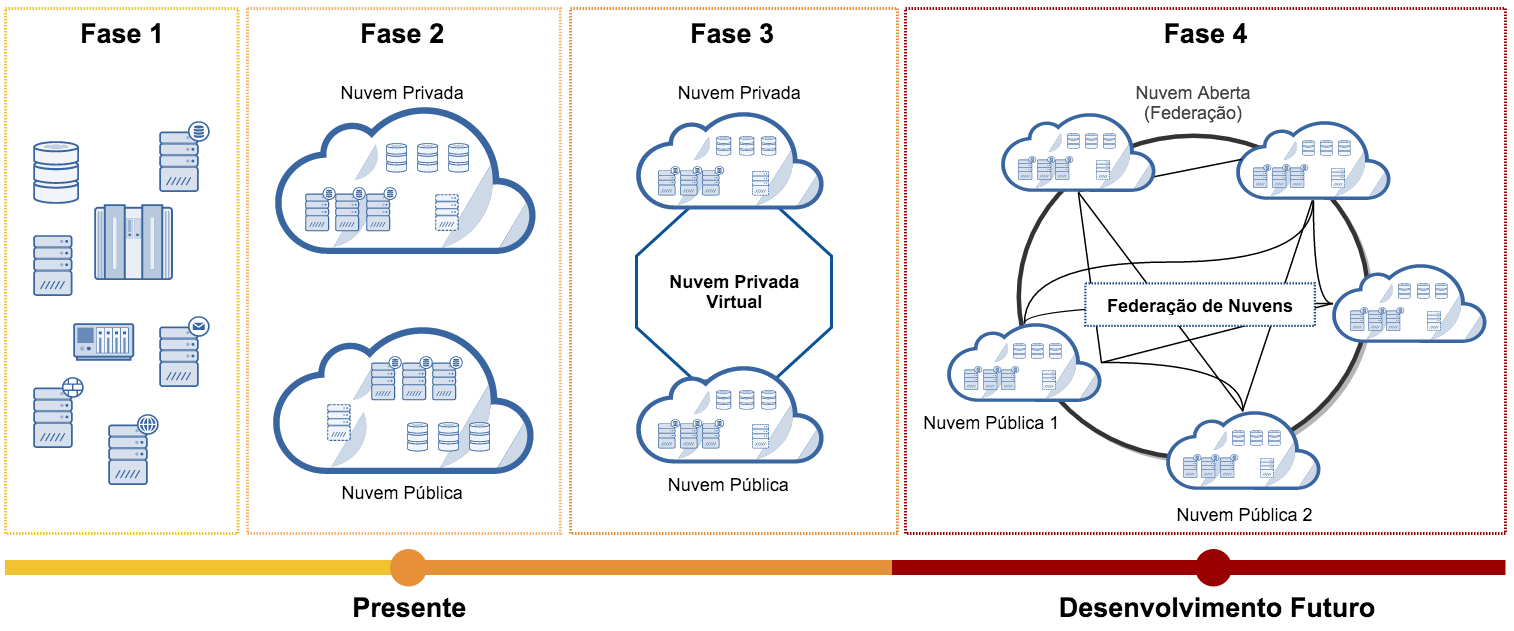
\includegraphics[scale=0.3]{fases_federacao.png}
	\caption{Fases da computação em nuvem, segundo White E. \textit{et al.} [26].}
	\label{fig:federacao_nuvens}
\end{figure}

A federação de nuvens passou por quatro fases. A Figura \ref{fig:federacao_nuvens} apresenta claramente essas quatro fases de implantação, as quais são"

\begin{itemize}
	\item \textbf{Primeira Fase:} É possível notar \textit{datacenters} desconexos, sem utilizar o conceito de nuvem computacional, ou seja, estão espalhados pelo mundo e realizam todo o trabalho sozinhos, contando apenas com a sua própria infraestrutura e mecanismo de gerenciamento. Assim, estão mais propensos à falhas e não compartilham recursos computacionais com outros \textit{datacenters};
    \item \textbf{Segunda Fase:} Nessa fase da computação em nuvem, as nuvens já possuem tecnologia e mecanismos para disponibilizar seus serviços pela Internet, estando acessíveis a usuários finais. É o que vemos em serviços como Dropbox (\textit{Software-as-a-Service}) [27], Amazon EC2 (\textit{Infrastructure-as-a-Service}) [28] ou Heroku (\textit{Platform-as-a-Service}) [29];
    \item \textbf{Terceira Fase:} As nuvens já conseguem compartilhar recursos entre si por meio de um provedor virtual que realiza todo o balanceamento das nuvens, de forma que nenhum provedor fique ocioso enquanto há outros que se encontram utilizando sua carga máxima de recursos. Celesti \textit{et al.} [20] as tipificou em duas definições: \textit{Home Clouds}, nuvens com sua capacidade computacional saturada e \textit{Foreign Clouds}, aquelas com recursos ociosos disponíveis e que podem ser utilizados por outras nuvens. Nesse caso, uma solicitação seria enviada para a nuvem com recursos ociosos, e esses seriam disponilizados para a nuvem sobrecarregada;
    \item \textbf{Quarta Fase:} Atualmente os provedores de serviços estão nessa última fase, na qual encontram-se as várias federações de nuvens espalhadas pelo mundo, trabalhando de forma interoperável entre si, ou seja, dividindo os seus recursos quando ociosos, e requisitando recursos quando saturados. Esse conceito de ``nuvem de federações'' forma um cenário no qual os recursos desperdiçados na nuvem são escassos, dada sua utilização por outros provedores. Isso traz um melhor balanceamento de carga, com poucos serviços indisponíveis por uma possível saturação, fazendo com que os usuários experimentem uma melhor experiência de aplicações hospedadas nas nuvens. 
\end{itemize}

\begin{center}
	\textbf{\small{imagem de uma federação de nuvens}}
\end{center}

Apesar das vantagens desse novo modelo de computação em nuvem, a implementação de tal cenário de federação de nuvens não é trivial, pois as nuvens são mais complexas do que os sistemas tradicionais. De fato, enquanto as nuvens são tipicamente compostas por recursos heterogêneo (diversos sistemas operacionais, configurações, poder computacional, latência de rede) e dinâmicos, os modelos existentes de federação são projetados para ambientes estáticos nos quais acordos prévios entre as partes são necessários para estabelecer a federação. Assim, a federação de nuvens precisa atender aos seguintes requisitos [20]:

\begin{itemize}
	\item \textbf{Automatismo e Escalabilidade:} Usando mecanismos de descoberta, a nuvem computacional com a utilização de recursos computacionais saturada deve ser capaz de escolher a melhor nuvem que satisfaça as suas exigências de recursos;
    \item \textbf{Segurança Interoperável:} Se faz necessária a integração de diferentes tecnologias de segurança entre nuvens computacionais, permitindo uma nuvem ser capaz de juntar-se à federação sem alterar as suas próprias políticas de segurança.
\end{itemize}


